\documentclass[12pt,titlepage]{article}\usepackage{graphicx, color}
%% maxwidth is the original width if it is less than linewidth
%% otherwise use linewidth (to make sure the graphics do not exceed the margin)
\makeatletter
\def\maxwidth{ %
  \ifdim\Gin@nat@width>\linewidth
    \linewidth
  \else
    \Gin@nat@width
  \fi
}
\makeatother

\IfFileExists{upquote.sty}{\usepackage{upquote}}{}
\definecolor{fgcolor}{rgb}{0.2, 0.2, 0.2}
\newcommand{\hlnumber}[1]{\textcolor[rgb]{0,0,0}{#1}}%
\newcommand{\hlfunctioncall}[1]{\textcolor[rgb]{0.501960784313725,0,0.329411764705882}{\textbf{#1}}}%
\newcommand{\hlstring}[1]{\textcolor[rgb]{0.6,0.6,1}{#1}}%
\newcommand{\hlkeyword}[1]{\textcolor[rgb]{0,0,0}{\textbf{#1}}}%
\newcommand{\hlargument}[1]{\textcolor[rgb]{0.690196078431373,0.250980392156863,0.0196078431372549}{#1}}%
\newcommand{\hlcomment}[1]{\textcolor[rgb]{0.180392156862745,0.6,0.341176470588235}{#1}}%
\newcommand{\hlroxygencomment}[1]{\textcolor[rgb]{0.43921568627451,0.47843137254902,0.701960784313725}{#1}}%
\newcommand{\hlformalargs}[1]{\textcolor[rgb]{0.690196078431373,0.250980392156863,0.0196078431372549}{#1}}%
\newcommand{\hleqformalargs}[1]{\textcolor[rgb]{0.690196078431373,0.250980392156863,0.0196078431372549}{#1}}%
\newcommand{\hlassignement}[1]{\textcolor[rgb]{0,0,0}{\textbf{#1}}}%
\newcommand{\hlpackage}[1]{\textcolor[rgb]{0.588235294117647,0.709803921568627,0.145098039215686}{#1}}%
\newcommand{\hlslot}[1]{\textit{#1}}%
\newcommand{\hlsymbol}[1]{\textcolor[rgb]{0,0,0}{#1}}%
\newcommand{\hlprompt}[1]{\textcolor[rgb]{0.2,0.2,0.2}{#1}}%

\usepackage{framed}
\makeatletter
\newenvironment{kframe}{%
 \def\at@end@of@kframe{}%
 \ifinner\ifhmode%
  \def\at@end@of@kframe{\end{minipage}}%
  \begin{minipage}{\columnwidth}%
 \fi\fi%
 \def\FrameCommand##1{\hskip\@totalleftmargin \hskip-\fboxsep
 \colorbox{shadecolor}{##1}\hskip-\fboxsep
     % There is no \\@totalrightmargin, so:
     \hskip-\linewidth \hskip-\@totalleftmargin \hskip\columnwidth}%
 \MakeFramed {\advance\hsize-\width
   \@totalleftmargin\z@ \linewidth\hsize
   \@setminipage}}%
 {\par\unskip\endMakeFramed%
 \at@end@of@kframe}
\makeatother

\definecolor{shadecolor}{rgb}{.97, .97, .97}
\definecolor{messagecolor}{rgb}{0, 0, 0}
\definecolor{warningcolor}{rgb}{1, 0, 1}
\definecolor{errorcolor}{rgb}{1, 0, 0}
\newenvironment{knitrout}{}{} % an empty environment to be redefined in TeX

\usepackage{alltt}

\usepackage{mcgill,palatino,fancyhdr}

\lhead{STAT201A -- Sec. 102}
\chead{HW \#8. }
\rhead{Steven Pollack -- 24112977}
\cfoot{\thepage}

\title{STAT201A -- Sec. 102 \\ Homework \#8. }
\author{Steven Pollack \\ 24112977}
\date{}

\begin{document}
\maketitle

\pagestyle{empty}
\newpage
\pagestyle{fancy}

\paragraph{\#1.}
\begin{proof}
Given a generic prediction, $W = g(X)$, and setting $h(X) = E(Y\given{X}) - W$, the MSE of $W$ is $E[(Y-W)^2]$ and can be rewritten as
\begin{align*}
E\left[(Y-W)^2\right] &= E\left( E\left[(Y-W)^2 \given{X}\right]\right) \\
&= E\left( E\left[ \set{ (Y- E(Y\given{X})) + h(X) }^2 \given{X} \right] \right) \\
&=E\left( E\left[ (Y-E(Y\given{X}))^2 \given{X} \right] \right) + 2E\left(E\left[ (Y-E(Y\given{X})) h(X) \given{X} \right] \right) + E\left(E \left[ h(X)^2 \given{X} \right] \right) \\
&= \var(Y\given{X}) + 2E\left(h(X) \underbrace{E\left[ Y-E(Y\given{X}) \given{X}\right]}_{=0}\right)  + E\left[ h(X)^2 \right]  \\
&= \var(Y \given{X}) + E\left[ h(X)^2 \right]
\end{align*}
Hence, the MSE of $Y$ and $W$ is minimized when $h(X) = 0 \EQ g(X) = E(Y \given{X})$. 
\end{proof}

\paragraph{\#2.}
\begin{proof}
Let $I_1$ indicate the event that a widget of the first kind is drawn, $I_2 = 1-I_1$ indicate for a widget of the second kind and set $Y$ to be the random variable that identifies the drawn widget. It follows that
\begin{align*}
E(Y \given{I_1}) = \mu I_1 + \nu I_2
\intertext{and }
\var(Y \given{I_1}) = \sigma^2 I_1 + \tau^2 I_2
\end{align*}
Thus, the law of iterated expectations says that
\[
E(Y) = E(E(Y\given{I_1})) = \frac{\mu + 2 \nu}{3}
\]
and our iterated variance rule shows that
\begin{align*}
\var(Y) &= E(\var(Y\given{I_1})) + \var(E(Y\given{I_1})) \\
&= E\left(\sigma^2 I_1 + \tau^2 I_2\right) + \var\left( \mu I_1 + \nu I_2 \right) \\
&= \frac{\sigma^2 + 2 \tau^2}{3} + \mu^2\var(I_1) + \nu^2 \var(I_2) +2\mu\nu\cov(I_1, I_2) \\
&= \frac{3(\sigma^2 + 2 \tau^2) + 2(\mu - \nu)^2}{9}
\end{align*}
\end{proof}

\paragraph{\#3.} Consider $B \sim$ HypGeo$(b_0 + w_0, b_0, d)$, and $\beta$ the number of black balls in a sample of size $n$. Then $\beta \sim$ HypGeo$(N, b+B, n)$, where $N= d + b+ w$. Then, $E(\beta \given{B}) = n \frac{b+B}{N}$ and
\begin{align*}
 E(\beta) &= E(E(\beta\given{B})) \\
&= \frac{n}{N}E(b+B) \\
&= \frac{n}{N}(b + E(B)) \\
&= \frac{n}{N}\left(b + d\frac{b_0}{b_0+w_0}\right)
\end{align*}
and
\begin{align*}
\var(\beta) &= \var(E(\beta\given{B})) + E(\var(\beta\given{B})) \\
&= \var\left(n\frac{b+B}{N}\right) + E\left( n \frac{b+B}{N}\frac{d+w-B}{N}{\frac{N-n}{N-1}} \right) \\
&= \frac{n^2}{N^2}\var(b+B) + \frac{n}{N^2}{\frac{N-n}{N-1}} E((b+B)(d+w-B)) \\
&=\frac{n^2}{N^2}\var(B) + \frac{n}{N^2}{\frac{N-n}{N-1}}  E(bd +(d+w-b)B-B^2) \\
&= \frac{n^2}{N^2}\var(B) + \frac{n}{N^2}{\frac{N-n}{N-1}} \left( bd +(d+w-b)E(B)-E(B^2)\right) \\
&= \frac{n^2}{N^2}\var(B) + \frac{n}{N^2}{\frac{N-n}{N-1}} \left( bd +(d+w-b)E(B)-\var(B) - E(B)^2\right) \\
&=\frac{n}{N^2}\left(n - \frac{N-n}{N-1}\right)\var(B) + \frac{n}{N^2}{\frac{N-n}{N-1}} \left( bd +(d+w-b)E(B) - E(B)^2\right) \\
&=\frac{n(n-1)}{N(N-1)}\var(B) + \frac{n}{N^2}{\frac{N-n}{N-1}} \left( bd +(d+w-b)E(B) - E(B)^2\right)
\end{align*}
where
\[
\var(B) = d \left(\frac{b_0}{b_0+w_0}\right) \left(\frac{w_0}{b_0 + w_0}\right) \left(\frac{b_0 + w_0 - d}{b_0 + w_0 -1} \right)
\]

\paragraph{\#4.}
\begin{enumerate}
\item Given $X, X_1, X_2, \ldots \iid F_{X}$, where $X_i$ have MGF $\psi_{X}$, 
\begin{align*}
\psi_{S}(t) &= E\left[ e^{tS} \right] \\
&= E\left[ E\left( e^{t\SUM{i}{1}{N}X_i} \biggl| {N} \right) \right] \\
&= E\left[ \psi_{X}(t)^{N} \right] \\
&= E\left[ \exp\set{ N \log(\psi_{X}(t))} \right] \\
&= \psi_{N}(\log(\psi_{X}(t))
\end{align*}
where the third equality comes from the fact that $E\left(\exp\set{t\SUM{i}{1}{N}X_i}\given{N=n}\right) = \psi_{X}(t)^{n}$. 
\item Given $N \sim$ Poisson$(\lambda)$:
\begin{align*}
\psi_{N}(t) &= E(e^{tN}) \\
&= \SUM{n}{0}{\infty} e^{tn} e^{-\lambda} \frac{\lambda^n}{n!} \\
&= e^{-\lambda} \SUM{n}{0}{\infty} \frac{(e^t\lambda)^n}{n!} \\
&= e^{-\lambda} e^{e^t \lambda} \\
&= \exp\set{\lambda(e^t-1)}
\end{align*}
\item For $I$ an indicator random variable with $P(I=1) = p$, the mgf of $I$ is: \[\psi_{I}(t) = 1 + p(e^{t}-1)\]
Putting this all together, if we toss a coin $N \sim$ Poisson$(\lambda)$ times, where each head has probability $p$, then $X$, the number of heads in $N$ tosses looks like $\SUM{i}{1}{N} I_i$, where $I_i$ indicates a heads on the $i^{th}$ toss. Thus, 
\begin{align*}
\psi_{X}(t) &= \psi_{N}(\log(\psi_{I_1}(t))) \\
&= \exp\set{\lambda(\exp\set{\log\psi_{I_1}(t)}-1)} \\
&= \exp\set{\lambda(\psi_{I_1}(t) - 1)} \\
&= \exp\set{\lambda p(e^t - 1)}
\end{align*}
which shows that $X \sim $ Poisson($\lambda p$). 
\end{enumerate}

\paragraph{\#5.}
\begin{enumerate}
\item Let $\Theta \sim \beta$eta($r,s$) be the probability of getting a heads (endowed with a $\beta(r,s)$ prior density), and note that our experiment follows $X \sim$ Geo$(\Theta$). Hence, our likelihood is $P(X = k \given{\Theta \in d\theta}) = (1-d\theta)^{k-1}d\theta$ and $P(\Theta \in d\theta) \propto d\theta^{r-1}(1-d\theta)^{s-1}$. Using the formula, posterior $\propto$ likelihood $\times$ prior, we have
\begin{align*}
P(\Theta \in d\theta \given{X = k}) &\propto P(X = k \given{\Theta \in d\theta}) \cdot P(\Theta \in d\theta) \\
&\propto d\theta^{r}(1-d\theta)^{s+k-2}
\end{align*}
Which means our posterior density is $\beta$eta$(r+1,s+k-1)$, making the beta densities are a family of conjugate priors, here. 
\item For a fixed $r,s$ we see that increasing $k$ puts more mass to the left of 1/2, which makes sense: a heavier ``head'' implies a lower probability of flipping heads, and hence a longer waiting time. 
\end{enumerate}

\paragraph{\#6.} 



\begin{enumerate}
\item Set $f_{\rho}(u,v) = \rho u + \sqrt{1-\rho^2} v$, and note that for $-1\leq \rho \leq 1$, and $U, V \sim$ N(0,1) with $U \orth V$, $(U, f(U,V))$ is distributed according to the standard bivariate normal distribution with correlation $\rho$. Thus, if we take $X \sim$ N($\mu_{X}$, $\sigma_{X}^{2}$), and $V \sim$ N($\mu_{Y}$, $\sigma_{Y}^{2}$), $X \orth V$, then 
\[
\left(\frac{X-\mu_{X}}{\sigma_{X}}, f_{\rho}\left(\frac{X-\mu_{X}}{\sigma_{X}}, \frac{V-\mu_{Y}}{\sigma_{Y}}\right) \right) \sim N\left(\mu=(0,0), \Sigma=
\begin{pmatrix}
1 & \rho \\
\rho & 1 
\end{pmatrix}
\right)
\]
Hence, if we perform the standard shift and scale, we'll get
\[
\left(X, \sigma_{Y} f_{\rho}\left(\frac{X-\mu_{X}}{\sigma_{X}}, \frac{V-\mu_{Y}}{\sigma_{Y}}\right) + \mu_{Y} \right) \sim N\left(
\mu=
\begin{pmatrix}
\mu_{X} \\ \mu_{Y}
\end{pmatrix}, \Sigma = 
\begin{pmatrix} 
\sigma_{X} & 0 \\
0 & \sigma_{Y}
\end{pmatrix} 
\begin{pmatrix}
1 & \rho \\
\rho & 1 
\end{pmatrix}
\begin{pmatrix} 
\sigma_{X} & 0 \\
0 & \sigma_{Y}
\end{pmatrix}
\right)
\]
That is, if $Y = \sigma_{Y}f_{\rho}\left(\frac{X-\mu_{X}}{\sigma_{X}}, \frac{V-\mu_{Y}}{\sigma_{Y}}\right) + \mu_{Y} $, then
\[
(X,Y) \sim N\left(
\mu=
\begin{pmatrix}
\mu_{X} \\ \mu_{Y}
\end{pmatrix}, \Sigma = 
\begin{pmatrix} 
\sigma_{X}^{2} & \rho \sigma_{X} \sigma_{Y} \\
\rho \sigma_{X} \sigma_{Y} & \sigma_{Y}^{2}
\end{pmatrix}
\right)
\]
So, putting this machinery to good use, let $X = MSAT$, with $\mu_{X} = 500$, $\sigma_{X} = 90$, and $Y = VSAT$ with $\mu_{Y} = 480$ and $\sigma_{Y} = 100$ and suppose the correlation between $X$ and $Y$ is $\rho = 0.5$. Then, the above construction shows that 
\begin{align*}
P(MSAT > VSAT) &= P( X > \sigma_{Y} f_{\rho}(X^{*},V^{*}) + \mu_{Y}) \\
&= P( X > \sigma_{Y}\rho X^{*} + \sigma_{Y} \sqrt{1-\rho^2} V^{*} + \mu_{Y}) \\
&= P\left(\frac{X - \sigma_{Y} \rho X^{*} - \mu_{Y}}{\sigma_{Y}\sqrt{1-\rho^2}} > V^{*}\right) \\
&= \int_{x=-\infty}^{\infty} \int_{v=-\infty}^{g(x,\rho,\sigma_{X},\mu_{Y},\sigma_{Y})} f_{X,V}(x,y) \, dv \, dx \\
&= \int_{x=-\infty}^{\infty} f_{X}(x) \int_{v=-\infty}^{g(x,\rho,\sigma_{X},\mu_{Y},\sigma_{Y})} f_{V^{*}}(v) \, dv \, dx \\
&= \int_{x=-\infty}^{\infty} f_{X}(x) \Phi\left(\frac{x - \sigma_{Y} \rho \sigma_{X}^{-1} (x-\mu_{X}) - \mu_{Y}}{\sigma_{Y}\sqrt{1-\rho^2}}\right) \, dx
\end{align*}
Where the fifth equation is justified since $X \orth V$, by assumption and thus $X \orth V^{*}$. Plugging in the appropriate parameters in the equation and having R run the integral, we find
\[
P(MSAT > VSAT) \approx 0.5830323
\]
\item Using the setup above, we have that for $MSAT = 550$, our random vector, $(MSAT,VSAT)$, looks like
\[
(550, \sigma_{Y}f_{\rho}(550^{*},V^{*}) + \mu_{Y}) 
\]
which has normal distribution with mean = 507.7778 and sd = 86.6025. Thus, 
\begin{align*}
P(MSAT > VSAT \given{MSAT=550}) &= P(550 > VSAT \given{MSAT=550}) \\
&= \Phi\left(\frac{550-507.7778}{86.6025}\right)\\
&\approx 0.687062
\end{align*}
\end{enumerate}

\paragraph{\#7.}
\begin{proof}
\begin{enumerate}
\item Consider the experiment where we have two particles of type $x$ and $y$ and their frequency of appearance follows $X \sim$ Exp($\lambda$) and $Y \sim$ Exp($\mu$) for types $x$ and $y$, respectively. If $I$ indicates on the event that a particle of type $y$ appearance first, then $E(I) = P(X > Y)$. But, using the tower rule
\[
E(I) = E[E(I \given{Y})] = E[ e^{-\lambda Y} ] = \psi_{Y}(-\lambda) = \left(1 + \frac{\lambda}{\mu}\right)^{-1} = \frac{\mu}{\mu+\lambda}
\]
since
\[
E(I\given{Y\in (y-dy,y+dy) }) = P(X > y) = \int_{y}^{\infty} \lambda e^{-\lambda t} \, dt = e^{-\lambda y} 
\]
and $\psi_{Y}(t) = (1-t/\mu)^{-1}$. This answer still makes sense for $\mu =\lambda$, since in this instance, both particles have the same frequency of occurrence, so it's 50/50 that you'll get one over the other.
\item From the method of MGF's we have that $\psi_{cY}(t) = \psi_{Y}(ct) = (1-t/(\mu/c))^{-1}$, hence $cY \sim$ Exp($\mu/c$), and performing the entire argument above with $Y' = cY$, we have 
\[
P(X > cY) = \frac{\mu/c}{\mu/c+\lambda} = \frac{\mu}{\mu + c\lambda}
\]
\item From b)
\[
P(X > cY) =  P(X/Y > c) = \frac{\mu}{\mu + c\lambda} \EQ F_{X/Y}(c) = 1 - \frac{\mu}{\mu+c\lambda} = \frac{c\lambda}{\mu + c \lambda}
\]
\item To find the medium, we want $m$ such that $F_{X/Y}(m) = 50\%$. So, 
\[
F_{X/Y}(m) = \frac{1}{2} \EQ \frac{m\lambda}{\mu + m\lambda} = \frac{1}{2} \EQ 2m \lambda = \mu + m\lambda \EQ m = \frac{\mu}{\lambda}
\]
Since the median of $Y$ is $m_{Y} = \ln(2)/\mu$, we have that $m = m_{X}/m_{Y}$. Also, $E(Y) = \mu^{-1}$ shows that $m = E(X)/E(Y)$.
\item It's a trap! If you differentiate $F_{X/Y}$ with respect to $c$, you recover the density of $X/Y$:
\[
f_{X/Y}(c) = \frac{\lambda \mu}{(\mu+\lambda c)^2} = \Theta\left(\frac{1}{c^2}\right)
\]
Hence, $E(X/Y) = \int_{0}^{\infty} c f_{X/Y}(c) \, dc = + \infty$, since $c f_{X/Y}(c) = \Theta(c^{-1})$. Thus, $X/Y$ has a median but no density!
\end{enumerate}
\end{proof}

\paragraph{\#8.}
\begin{proof}
\begin{enumerate}
\item For $X \sim \Gamma$amma($r,\lambda$), $\mu_{X} = r/\lambda$ and $\sigma_{X}^{2} = r/\lambda^2$, hence
\[
r = \mu_{X} \lambda = \sigma_{X}^{2} \lambda^2 \EQ r= \frac{\mu_{X}^2}{\sigma_{X}^2}
\]
So, we may as well try estimating $r$ via $\hat{r} = \hat{\mu}_{1}^{2}/(\hat{\mu}_{2} - \hat{\mu}_{1}^{2})$. My rationale for this is that $\hat{\mu}_{1} \approx \mu_{X}$ and $\hat{\mu}_{2} - \hat{\mu}_{1}^{2} \approx E(X^2) - E(X)^2 = \sigma_{X}^{2}$ for $n$ large, so hopefully the limit of their ratio will tend to $\mu_{X}/\sigma_{X}^{2} = r$. By this same rationale, we might try using $\hat{\lambda} = \hat{\mu}_{1}/(\hat{\mu}_{2} - \hat{\mu}_{1}^{2})$. 
\item Using the following code

\begin{knitrout}
\definecolor{shadecolor}{rgb}{0.969, 0.969, 0.969}\color{fgcolor}\begin{kframe}
\begin{alltt}
\hlfunctioncall{set.seed}(112)

r <- \hlfunctioncall{round}(\hlfunctioncall{runif}(n=1,min=2,max=5),digits=2) \hlcomment{# r = 3.13}
lambda <- \hlfunctioncall{round}(\hlfunctioncall{runif}(n=1,min=1,max=2),digits=2) \hlcomment{# lambda = 1.92}

n <- 100
X <- \hlfunctioncall{rgamma}(n=n,shape=r,rate=lambda)
mu_hat_1 <- (1/n)*\hlfunctioncall{sum}(X^1)
mu_hat_2 <- (1/n)*\hlfunctioncall{sum}(X^2)

r_hat <-  (mu_hat_1^2)/(mu_hat_2 - mu_hat_1^2) \hlcomment{# r_hat = 4.097228}
\hlfunctioncall{print}(\hlfunctioncall{abs}(r-r_hat))
\end{alltt}
\begin{verbatim}
[1] 0.9672
\end{verbatim}
\begin{alltt}
lambda_hat <- mu_hat_1/(mu_hat_2 - mu_hat_1^2) \hlcomment{# lambda_hat = 2.603451}
\hlfunctioncall{print}(\hlfunctioncall{abs}(lambda-lambda_hat))
\end{alltt}
\begin{verbatim}
[1] 0.6835
\end{verbatim}
\end{kframe}
\end{knitrout}

and
\begin{knitrout}
\definecolor{shadecolor}{rgb}{0.969, 0.969, 0.969}\color{fgcolor}\begin{kframe}
\begin{alltt}
p1 <- \hlfunctioncall{ggplot}(\hlfunctioncall{data.frame}(x=\hlfunctioncall{c}(0,5))) +
  \hlfunctioncall{geom_histogram}(\hlfunctioncall{aes}(x = X, y = ..density..), alpha = 0.25,
                 binwidth=0.3333) +
  \hlfunctioncall{stat_function}(fun=dgamma, arg=\hlfunctioncall{list}(shape=r,rate=lambda),
                colour=\hlstring{"darkgreen"}) 
\hlfunctioncall{print}(p1)
\end{alltt}
\end{kframe}
\end{knitrout}


\begin{figure}[htb]
\centering
\begin{knitrout}
\definecolor{shadecolor}{rgb}{0.969, 0.969, 0.969}\color{fgcolor}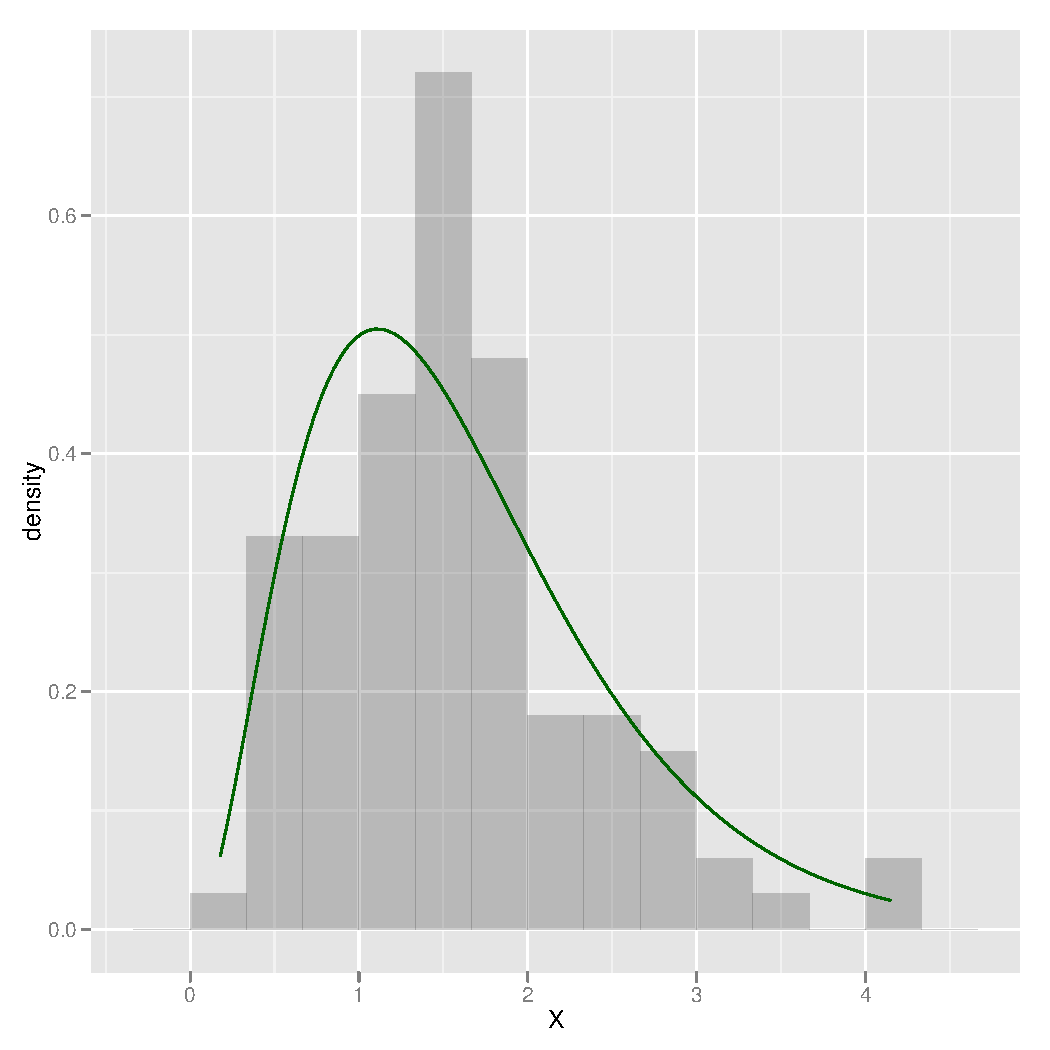
\includegraphics[width=0.65\textwidth]{figure/unnamed-chunk-1} 
\end{knitrout}
\caption{Histogram of $n = 100$ iid samples from $\Gamma$($r$=3.13, $\lambda$=1.92) with density overlayed.}
\label{fig:hist_and_density}
\end{figure}

We can see that the histogram in figure \ref{fig:hist_and_density} resembles the density of our sample distribution (though, it could stand to resemble it more closely); however, I'm remiss to say my estimators are not very close to their targets\ldots

\item



The mean our 1000 estimations of $r$ and $\lambda$ are 3.2619 and 2.0066, respectively. The SD of our the 1000 estimations is 0.5382 and 0.349. See figure \ref{fig:estimators_for_100} for histograms of the estimators.

\begin{figure}[ht!]
\centering
\begin{knitrout}
\definecolor{shadecolor}{rgb}{0.969, 0.969, 0.969}\color{fgcolor}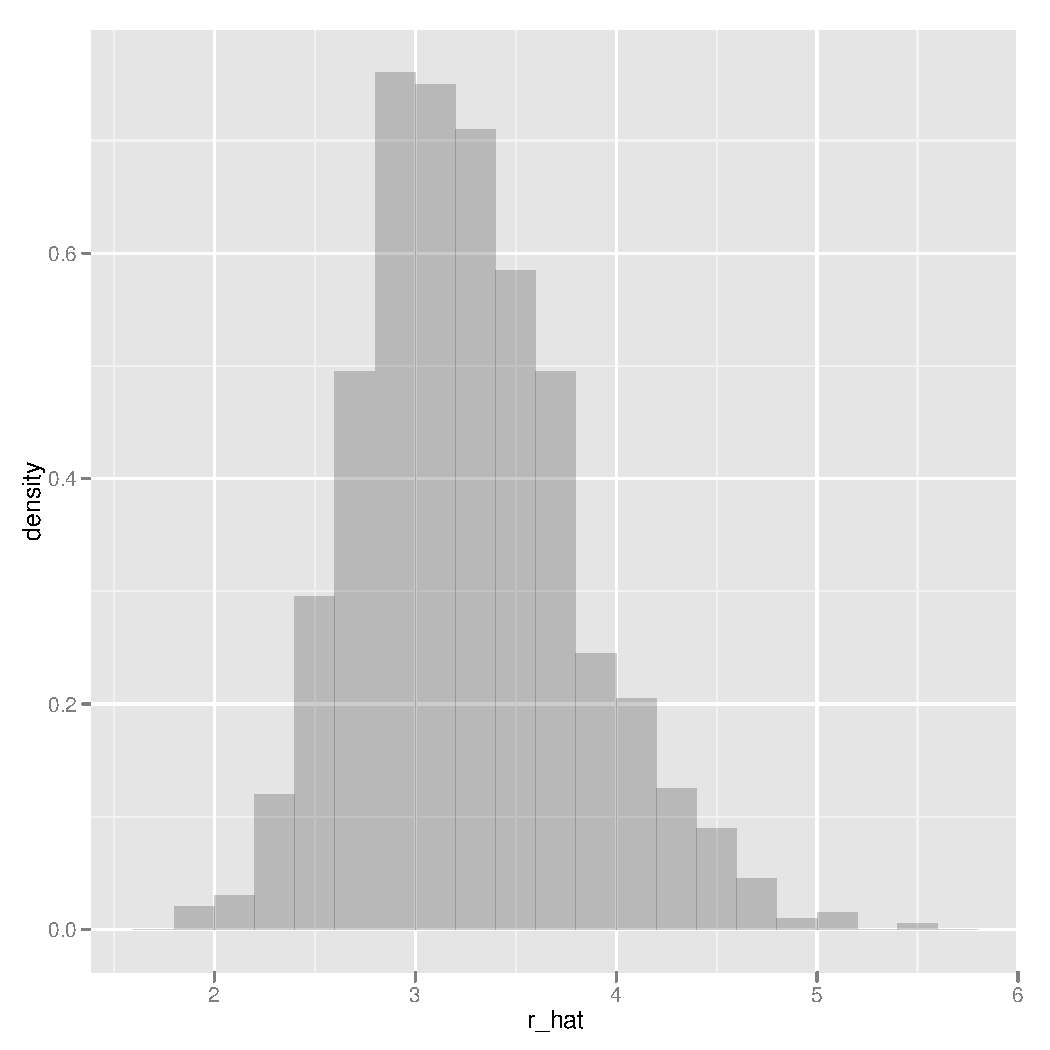
\includegraphics[width=0.45\textwidth]{figure/partDPlots} 
\end{knitrout}
\begin{knitrout}
\definecolor{shadecolor}{rgb}{0.969, 0.969, 0.969}\color{fgcolor}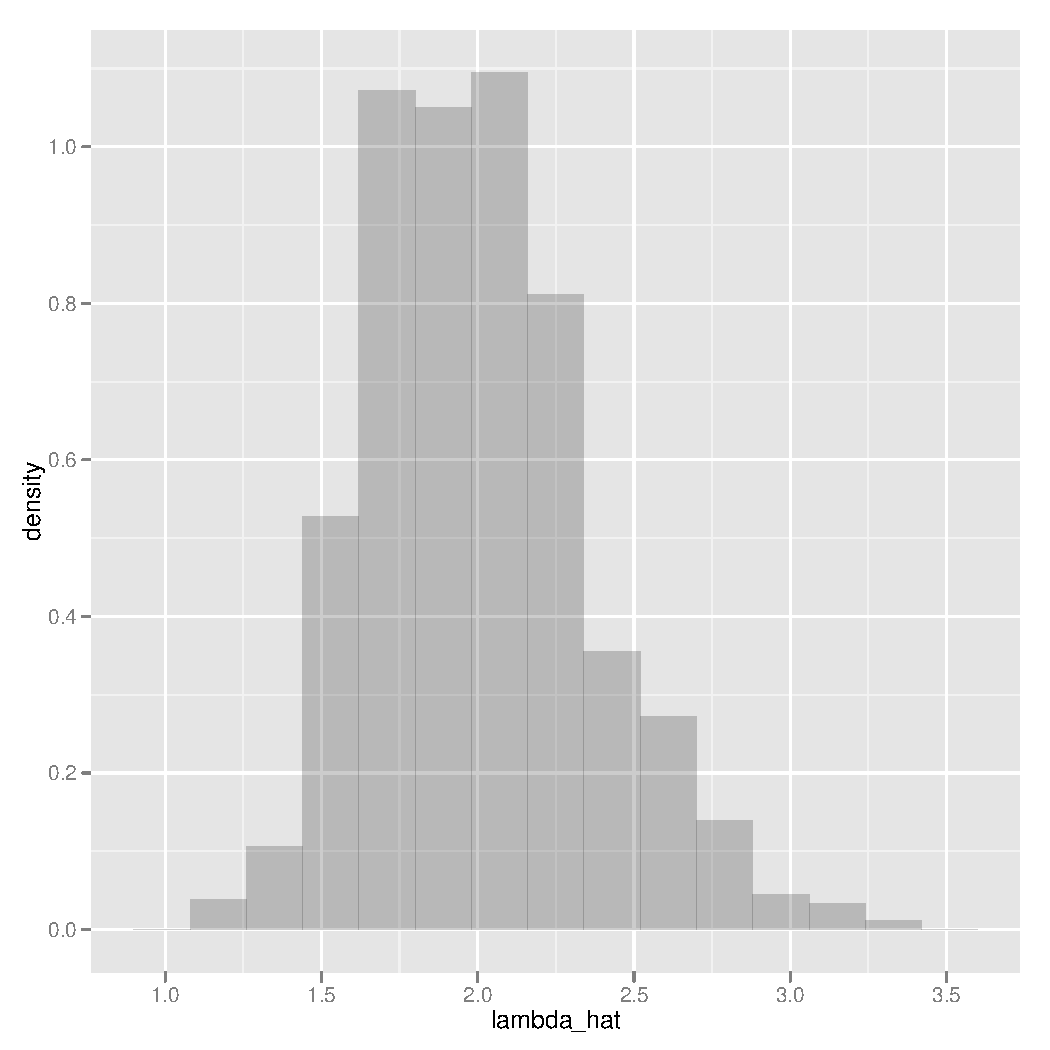
\includegraphics[width=0.45\textwidth]{figure/partDPlots2} 
\end{knitrout}

\caption{Histograms for $\hat{r}$ and $\hat{\lambda}$ when $n=100$}
\label{fig:estimators_for_100}
\end{figure}
\end{enumerate}
\end{proof}

\paragraph{\#9.} Using the following code

\begin{knitrout}
\definecolor{shadecolor}{rgb}{0.969, 0.969, 0.969}\color{fgcolor}\begin{kframe}
\begin{alltt}
n <- 1e3
times <- 1e3

new_estimators <- \hlfunctioncall{t}(\hlfunctioncall{mapply}(FUN=generateEstimators,
                           n=\hlfunctioncall{rep}(n,times=times),
                           r=\hlfunctioncall{rep}(r,times=times),
                           lambda=\hlfunctioncall{rep}(lambda,times=times)))

r_hat <- new_estimators[,1]
lambda_hat <- new_estimators[,2]
\end{alltt}
\end{kframe}
\end{knitrout}


The mean our \textit{new} 1000 estimations of $r$ and $\lambda$ are 3.1447 and 1.9287, respectively. The SD of our the 1000 estimations is 0.1654 and 0.1062. It seems that our estimators are, indeed, converging to their targets. I'm willing to say this is most likely a consequence of the fact that $\hat{\mu}_{k} \to E(X^k)$ with whatever speed the weak-law of large numbers affords us. Figure \ref{fig:estimators_for_1000} shows the histograms for these new estimates. Notice that they more closely resemble bell curves.

\begin{figure}[ht!]
\centering
\begin{knitrout}
\definecolor{shadecolor}{rgb}{0.969, 0.969, 0.969}\color{fgcolor}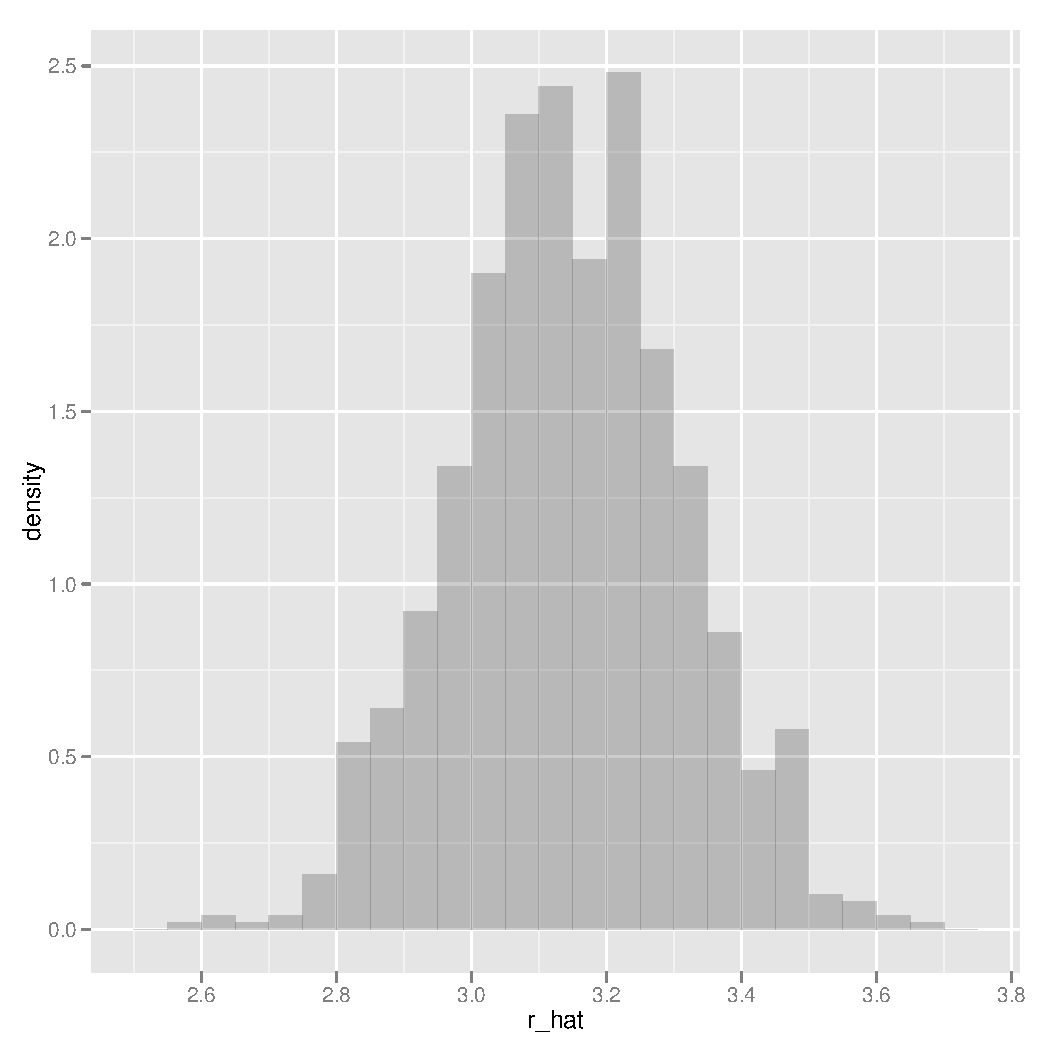
\includegraphics[width=0.45\textwidth]{figure/prob9Plots} 
\end{knitrout}
\begin{knitrout}
\definecolor{shadecolor}{rgb}{0.969, 0.969, 0.969}\color{fgcolor}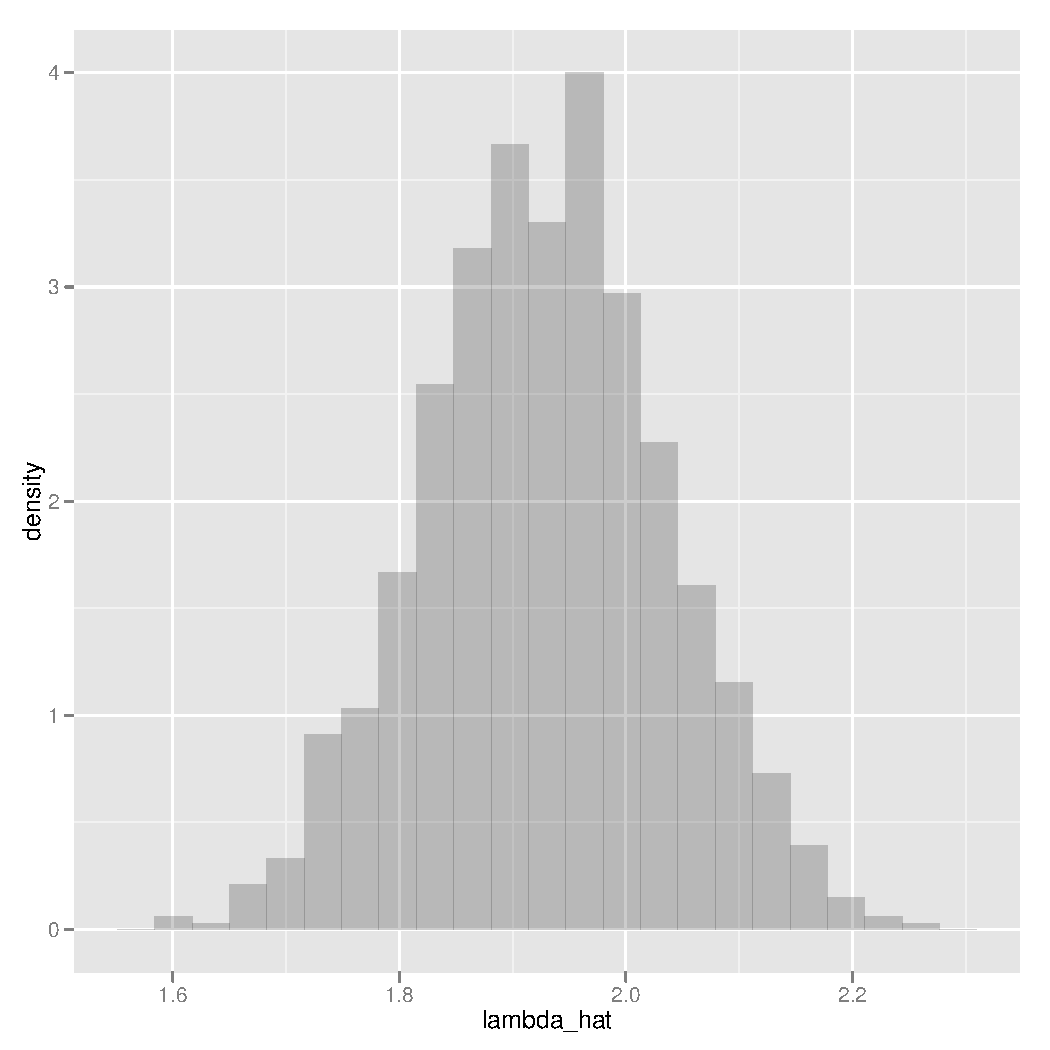
\includegraphics[width=0.45\textwidth]{figure/prob9Plots2} 
\end{knitrout}

\caption{Histograms for $\hat{r}$ and $\hat{\lambda}$ when $n=1000$}
\label{fig:estimators_for_1000}
\end{figure}

\paragraph{\#10.}
The following code performs the bootstrap algorithm, based on the preceding chunk's result:
\begin{knitrout}
\definecolor{shadecolor}{rgb}{0.969, 0.969, 0.969}\color{fgcolor}\begin{kframe}
\begin{alltt}
r_hat1 <- r_hat[1]
lambda_hat1 <- lambda_hat[1]

bootstrap_estimators <- \hlfunctioncall{t}(\hlfunctioncall{mapply}(FUN=generateEstimators,
                       n=\hlfunctioncall{rep}(n,times=times), 
                       r=\hlfunctioncall{rep}(r_hat1,times=times),
                       lambda=\hlfunctioncall{rep}(lambda_hat1,times=times)))

r_hat_bootstrap <- bootstrap_estimators[,1]
lambda_hat_bootstrap <- bootstrap_estimators[,2]

\end{alltt}
\end{kframe}
\end{knitrout}


And we find the new bootstrap estimators $\hat{\hat{r}}$ and $\hat{\hat{\lambda}}$ to have means and SD's 2.8622, 0.1498 and 1.7577, 0.0988. Note that our original $\hat{r} = 2.8851$ and $\hat{\lambda} = 1.7675$, so our bootstrap estimators do a very good job mimicing the original estimators. 

The central 95\% of $\hat{\hat{r}}$'s distribution is in (2.5797,3.1495), and the central 95\% of $\hat{\hat{\lambda}}$ is in (1.5668,1.9458). A simple inspection of figure \ref{fig:estimators_for_1000} shows that these intervals pretty much capture the same information as the distribution of $\hat{r}$ and $\hat{\lambda}$, so we can be confident that our estimands ($r,\lambda$) can be estimated via $\hat{\hat{r}}$ and $\hat{\hat{\lambda}}$.

\begin{figure}[ht!]
\centering
\begin{knitrout}
\definecolor{shadecolor}{rgb}{0.969, 0.969, 0.969}\color{fgcolor}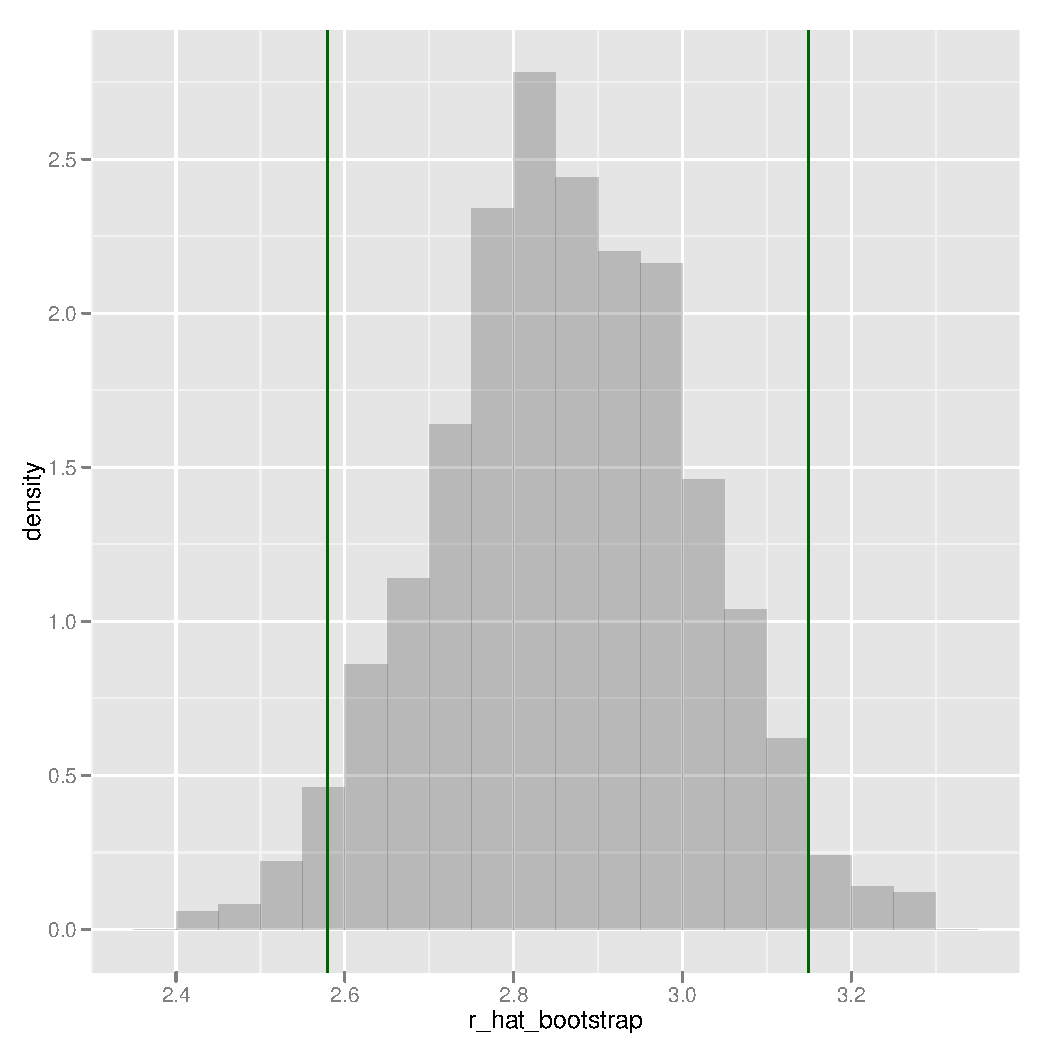
\includegraphics[width=0.45\textwidth]{figure/bootStrapPlots} 
\end{knitrout}
\begin{knitrout}
\definecolor{shadecolor}{rgb}{0.969, 0.969, 0.969}\color{fgcolor}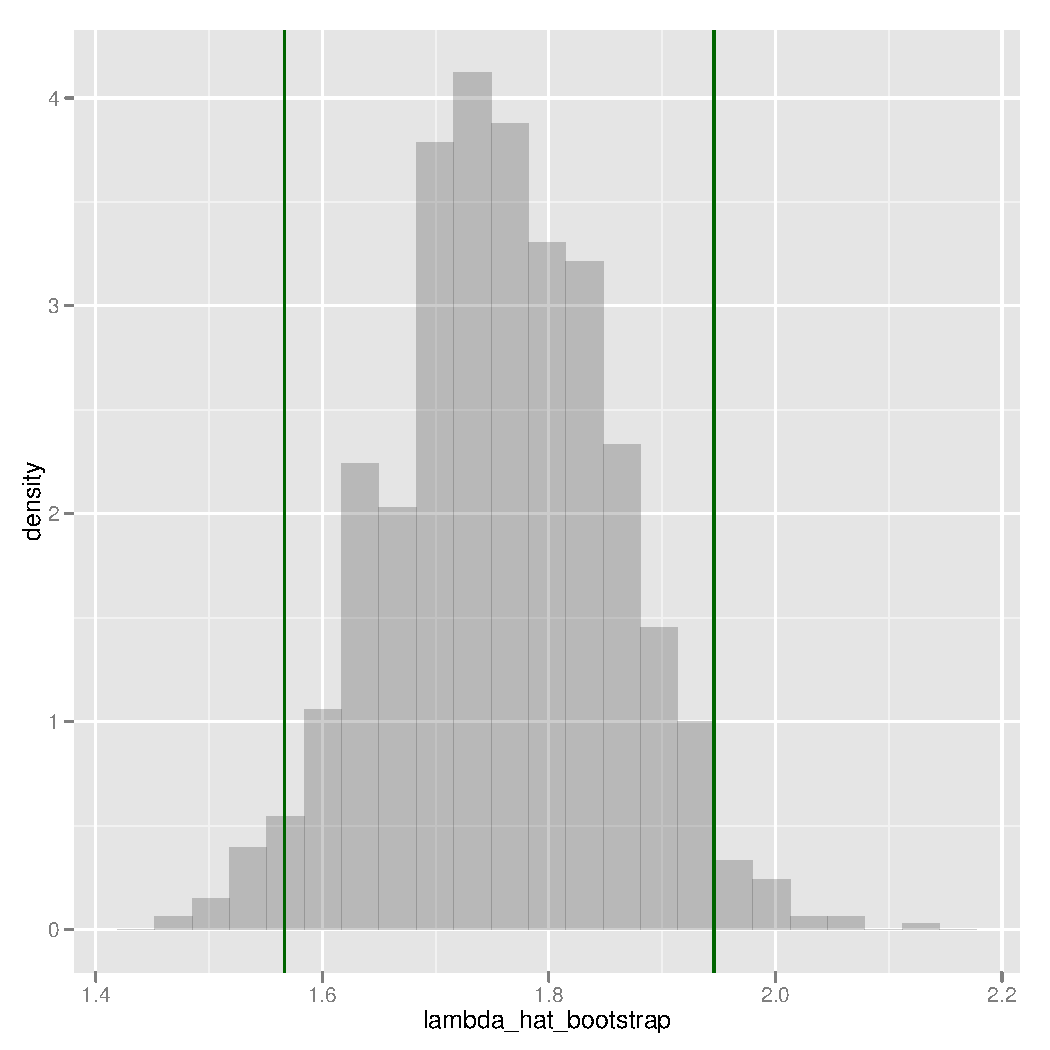
\includegraphics[width=0.45\textwidth]{figure/bootStrapPlots2} 
\end{knitrout}

\caption{Histograms for $\hat{\hat{r}}$ and $\hat{\hat{\lambda}}$ generated from bootstrap with vertical lines denoting the central 95\% of each distribution}
\label{fig:bootstrap_estimators_for_1000}
\end{figure}

\end{document}

